\documentclass[a4paper,11pt]{article}
\usepackage{amsmath,amsthm,amsfonts,amssymb,amscd,amstext,vmargin,graphics,graphicx,tabularx,multicol} 
\usepackage[francais]{babel}
\usepackage[utf8]{inputenc}  
\usepackage[T1]{fontenc} 
\usepackage{pstricks-add,tikz,tkz-tab,variations}
\usepackage[autolanguage,np]{numprint} 

\setmarginsrb{1.5cm}{0.5cm}{1cm}{0.5cm}{0cm}{0cm}{0cm}{0cm} %Gauche, haut, droite, haut
\newcounter{numexo}
\newcommand{\exo}[1]{\stepcounter{numexo}\noindent{\bf Exercice~\thenumexo} : \marginpar{\hfill /#1}}
\reversemarginpar


\newcounter{enumtabi}
\newcounter{enumtaba}
\newcommand{\q}{\stepcounter{enumtabi} \theenumtabi.  }
\newcommand{\qa}{\stepcounter{enumtaba} (\alph{enumtaba}) }
\newcommand{\initq}{\setcounter{enumtabi}{0}}
\newcommand{\initqa}{\setcounter{enumtaba}{0}}

\newcommand{\be}{\begin{enumerate}}
\newcommand{\ee}{\end{enumerate}}
\newcommand{\bi}{\begin{itemize}}
\newcommand{\ei}{\end{itemize}}
\newcommand{\bp}{\begin{pspicture*}}
\newcommand{\ep}{\end{pspicture*}}
\newcommand{\bt}{\begin{tabular}}
\newcommand{\et}{\end{tabular}}
\renewcommand{\tabularxcolumn}[1]{>{\centering}m{#1}} %(colonne m{} centrée, au lieu de p par défault) 
\newcommand{\tnl}{\tabularnewline}

\newcommand{\bmul}[1]{\begin{multicols}{#1}}
\newcommand{\emul}{\end{multicols}}

\newcommand{\trait}{\noindent \rule{\linewidth}{0.2mm}}
\newcommand{\hs}[1]{\hspace{#1}}
\newcommand{\vs}[1]{\vspace{#1}}

\newcommand{\N}{\mathbb{N}}
\newcommand{\Z}{\mathbb{Z}}
\newcommand{\R}{\mathbb{R}}
\newcommand{\C}{\mathbb{C}}
\newcommand{\Dcal}{\mathcal{D}}
\newcommand{\Ccal}{\mathcal{C}}
\newcommand{\mc}{\mathcal}

\newcommand{\vect}[1]{\overrightarrow{#1}}
\newcommand{\ds}{\displaystyle}
\newcommand{\eq}{\quad \Leftrightarrow \quad}
\newcommand{\vecti}{\vec{\imath}}
\newcommand{\vectj}{\vec{\jmath}}
\newcommand{\Oij}{(O;\vec{\imath}, \vec{\jmath})}
\newcommand{\OIJ}{(O;I,J)}


\newcommand{\reponse}[1][1]{%
\multido{}{#1}{\makebox[\linewidth]{\rule[0pt]{0pt}{20pt}\dotfill}
}}

\newcommand{\titre}[5] 
% #1: titre #2: haut gauche #3: bas gauche #4: haut droite #5: bas droite
{
\noindent #2 \hfill #4 \\
#3 \hfill #5

\vspace{-1.6cm}

\begin{center}\rule{6cm}{0.5mm}\end{center}
\vspace{0.2cm}
\begin{center}{\large{\textbf{#1}}}\end{center}
\begin{center}\rule{6cm}{0.5mm}\end{center}
}



\begin{document}
\pagestyle{empty}
\titre{Interrogation: Droite des milieux }{Nom :}{Prénom :}{Classe}{Date}


\exo{1,5} Compléter les théorèmes suivants :\\

\bi
\item Dans un triangle, la droite qui passe par le milieu d'un côté et qui est parallèle à un second côté, passe \reponse[1]\\

\item Dans un triangle, le segment qui joint les milieux de deux côtés mesure \reponse[2]\\

\item Dans un triangle, si une droite passe par les milieux de deux côtés, alors \reponse[2]\\


\ei

\exo{3}\\

ABC est un triangle. I est le milieu du segment [AB]. La droite parallèle à (BC) passant par I coupe la droite (AC) en J. La droite parallèle à la droite (AB) passant par J coupe la droite (BC) en K.\\

\q Faire une figure.\\

\vspace*{4cm}

\q Démontrer que le point K est le milieu du segment [BC].\\
\reponse[6]\\

\exo{2,5}

L'une des chèvres de M. Ségou est insupportable. Il décide de l'isoler du reste du troupeau et de construire une clôture entre deux arbres, placés au milieu de deux côtés de son champ triangulaire.\\

\begin{center}
\includegraphics[scale=1]{cloture.eps} 
\end{center}

Quelle devra être la longueur de cette clôture ? \textbf{Démontrer votre réponse.}\\
\reponse[7]\\


\exo{3} 

\initq \q Montrer que les droites (MN) et (GH) sont parallèles\\

\bmul{2}
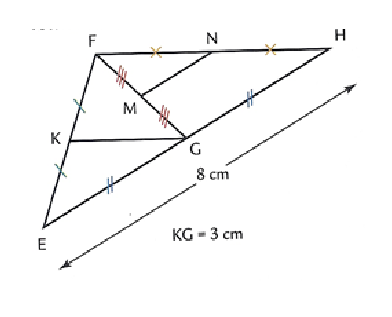
\includegraphics[scale=1]{droitepara.eps} 

\columnbreak

\noindent \reponse[7]

\emul

\q En déduire que (MN) et (EH) sont parallèles.\\
\reponse[2] 



\end{document}
